\documentclass[a4paper]{article}

%um nur aufgaben zu zeigen

\renewcommand{\title}{Aufgabenseminar\\ Klassische Mechanik}
\newcommand{\titleh}{Aufgabenseminar Klassische Mechanik}



\usepackage[noanswer]{exercise} 
\usepackage{../images/preamble}
\usepackage{rotating}
\usetikzlibrary{decorations.pathmorphing}
\usetikzlibrary{decorations.markings}
\usetikzlibrary{arrows}
\usetikzlibrary{shapes.geometric}
\usepackage{mathrsfs}
\newcommand{\midarrow}{\tikz \draw[-triangle 90] (0,0) -- +(.02,0);}
\usepackage{xcolor}
%\usepackage{draftwatermark}
%\SetWatermarkText{\textsc{Entwurf}}
%\SetWatermarkScale{6}
%\SetWatermarkColor{red!30}

\pagestyle{fancy}
\fancyhead[L]{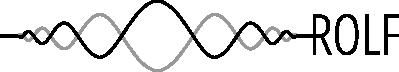
\includegraphics[width=2cm]{../images/logo_scaled.pdf}}
\fancyhead[R]{\textsc{\titleh}}


\renewcommand{\ExerciseHeader}{\textsf{\textbf{\ExerciseTitle} (\ExerciseOrigin)}\smallskip\newline}
\renewcommand{\AtBeginExercise}{\hspace{-0.66em}}


\begin{document}
	\vspace*{-1cm}
	\parbox{4cm}{\vspace{-0.2cm}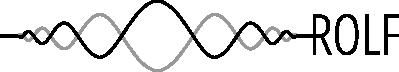
\includegraphics[width=5cm]{../images/logo_scaled.pdf}}
	\parbox{10.6cm}{\setstretch{2.0} \centering{ \huge \textsf{\title
			}}\\\url{pankratius.github.io/rolf}
			 }
		\vspace{0.5cm}
	
	

\thispagestyle{empty}


\noindent

\begin{Exercise}[label = adi, title = Pendel, difficulty = 5, origin = 1911]
	Wir betrachten ein harmonisches Pendel, desen Länge sich langsam ändert. Wie ändert sich die Amplitude der Schwingung?
\end{Exercise}
\begin{Exercise}[label = grassh, title = fauler Grashüpfer, origin = P.Gnädig, difficulty = 5]
	Ein fauler Grashüpfer möchte über einen Baumstumpf mit Radius $r = 20~\mathrm{cm}$ springen.\\
	Wie groß ist die dafür mindestens benötigte Geschwindigkeit, wenn der Luftwiderstand vernachlässigt werden kann?
\end{Exercise}
\begin{Answer}
	Bei minimaler Anfangsgeschwindigkeit sollte die Grashüpferbahn den Baumstamm in genau zwei Punkten symmetrisch zur Achse um den Baumstumpf berühren, und damit ihren Scheitelpunkt direkt auf dieser Achse haben, wie in Abbildung \ref{fig:grasshs} gezeigt ist. Dass die Bahn symmetrisch zur Symmetrieachse des Baums ist, liegt daran, dass sie reversibel sein sollte. Das bedeutet, dass es keinen Unterschied machen sollte, ob der Grashüpfer links oder rechts vom Baum losspringt, weshalb die Bahn symmetrisch sein muss. 
	%	\begin{figure}[h]
	%		\centering
	%		\begin{tikzpicture}[line cap=round,line join=round,>=triangle 45,x=1.0cm,y=1.0cm]
\clip(-3.573888715158432,-0.6284321850818549) rectangle (3.831338230521266,5.4106580654465875);
\draw [shift={(-3.,0.)}] (0,0) -- (0.:0.5107053065985999) arc (0.:72.38196924975453:0.5107053065985999) -- cycle;
\draw [shift={(-1.6166086789302696,3.1775297784800722)}] (0,0) -- (0.:0.5107053065985999) arc (0.:53.13793429316053:0.5107053065985999) -- cycle;
\draw [shift={(0.,2.)}] (0,0) -- (90.:0.5107053065985999) arc (90.:143.930590100419:0.5107053065985999) -- cycle;
\draw(0.,2.) circle (2.cm);
\draw [rotate around={90.:(0.,-25.3395997404539)}] (0.,-25.3395997404539) ellipse (29.719599740453898cm and 5.741326023857797cm);
\draw [->] (-1.6166086789302696,3.1775297784800722) -- (-0.76,4.32);
\draw (-1.6166086789302696,3.1775297784800722)-- (1.61660867893027,3.1775297784800722);
\draw (-1.6166086789302696,3.1775297784800722)-- (0.,2.);
\draw [->] (-3.,0.) -- (-2.6035486326210924,1.2484098166679993);
\begin{scriptsize}
\draw [fill=black] (-3.,0.) circle (2pt);
\draw [fill=black] (3.,0.) circle (2pt);
\draw [fill=black] (0.,2.) circle (2pt);
\draw [fill=black] (0.,0.) circle (2pt);
\draw [fill=black] (-1.6166086789302696,3.1775297784800722) circle (2pt);
\draw [fill=black] (1.61660867893027,3.1775297784800722) circle (2pt);
\draw [fill=black] (0.,4.38) circle (2pt);
%\draw [fill=black] (-0.76,4.32) circle (2.5pt);
\draw [fill=black] (0.,3.1775297784800722) circle (2pt);
%\draw [fill=black] (-2.6035486326210924,1.2484098166679993) circle (2.5pt);
\end{scriptsize}
\draw[thick] (-3.5,0)--(3.5,0);
\draw[thin,dashed](0,0)--(0,5);
\fill[pattern = north east lines] (-3.5,0)rectangle(3.5,-0.5);
\node at (-3.2,0.2){$A$};
\node at (3.2,0.2){$A^{\ast}$};
\node at (-2,3.1775297784800722){$B$};
\node at (2,3.1775297784800722){$B^{\ast}$};
\node at (0.5,2){$O$};
\node at (-1.25,2.5){$r$};
\node at (-2.25,0.2){$\alpha$};
\node at (-0.5,2.7) {$\theta$};
\node at (-0.9,3.4){$\theta$};
\node at (-1.8,3.8){$v_1$};
\node at (0.4,3.4){$C$};
\end{tikzpicture}
	%		\caption{Skizze der Grashüpferbahn}
	%		\label{fig:grasshs}		
	%	\end{figure}
	Es ist jetzt am einfachsten, wenn man zuerst die Bewegung des Grashüpfers von $B$ nach $B^{\ast}$ betrachtet. Die Geschwindigkeit des Grashüpfers in $B$ nennen wir $v_1$, und den Winkel, den die Grashüpfergeschwindigkeit mit dem Boden macht $\theta$.\\
	Dann wissen wir, dass die Wurfweite $s_w$ dieses schrägen Wurfes gegeben ist durch
	\begin{equation}\label{grassh:weite}
		s_w = \frac{2 v_1^2 \sin \theta \cos \theta}{g}.
	\end{equation}
	Geometrisch interpretiert muss diese Wurfweite $s_w$ genau die Strecke zwischen $B$ und $B^{\ast}$ sein. Wir versuchen jetzt, $\overline{BB^{\ast}}$ durch bekannte Parameter auszudrücken.\\
	Dazu macht es Sinn, wenn wir uns den Winkel $\angle COB$ anschauen. Wir wissen nämlich, dass die Geschwindigkeit (genauer: der Geschwindigkeits\textit{vektor}) tangiential zur Bahn sein muss, der Geschwindigkeitsvektor steht also senkrecht auf der Strecke $\overline{OB}$. Gleichzeitig ist das Dreieck $\Delta BOC$ ein rechtwinkliges, mit dem rechten Winkel $\angle BCO$. Damit ist also $\angle BOC = 180^\circ-90^\circ-\angle CBO = 90^\circ- \left(90^\circ- \theta\right) = \theta$.\\
	Jetzt können wir noch eine zweite Bedingung für $s_w$ aufstellen, allerdings in Abhängigkeit von $\theta$ und $r$. Das ist gut, weil wir dann einfach \eqref{grassh:weite} nehmen können, um $v_1$ auszurechen. Die Bedingung ist einfach, dass $s_w$ tatsächlich der Strecke $\overline{BB^\ast}$ entspricht. Es ist $\overline{BB^\ast} = 2 \overline{BC}$.\\
	Die Strecke $\overline{BC}$ können wir trigonometrisch durch $\theta$ im Dreieck $\Delta BOC$ ausrechnen. Dieses hat nämlich die Hypothenuse $r$, und der Winkel $\theta$ hat die Gegenkathete $\overline{BC}$. Also ist $\overline{BC} = r\cdot \sin \theta$. Damit haben wir jetzt die zweite Bedingung für $s_w$,
	\begin{equation}\label{grassh:weite2}
		s_w = \overline{BB^\ast} = 2 \overline{BC} = 2 r\cdot \sin \theta.
	\end{equation}
	Setzten wir \eqref{grassh:weite} und \eqref{grassh:weite2} gleich, kommen wir auf
	\begin{equation}\label{grassh:v2}
		\frac{2v_1^2\sin \theta \cos \theta}{g} = 2 r\cdot \sin \theta \Rightarrow v_1 = \sqrt{\frac{rg}{\cos\theta}}.
	\end{equation}
	Wir können jetzt die Energieerhaltung benutzten, um daraus die tatsächliche Anfangsgeschwindigkeit $v_0$ auszurechnen.\\
	Dazu brauchen wir aber noch die Höhe $h_B$ von Punkt $B$ überhalb des Bodens. Auch die können wir wieder durch $\theta$ ausrechnen. Die Höhe setzt sich nämlich zusammen aus der Höhe des Kreismittelpunkts $O$ über dem Boden (also dem Radius $r$) und der Strecke $\overline{OC}$. Die ist aber gerade die Ankathete zu $\theta$ im Dreieck $\Delta BOC$, sodass wir schreiben können $h_b = r + r\cos \theta = r\cdot\left(1+\cos \theta \right).$\\
	Die Energieerhaltung setzt nun die kinetische Energie am Punkt $A$ mit der Summe aus potentieller und kinetischer Energie in $B$ gleich, also
	\begin{equation}\label{grassh:coe}
		m\frac{v_0^2}{2} = m \frac{v_1^2}{2} + m g h_B\Rightarrow v_0^2 = \underbrace{\frac{rg}{\cos\theta}}_{\mathrm{aus}~\eqref{grassh:v2}} + 2g \underbrace{r\left(1+\cos \theta\right)}_{=h_B} =2 rg\cdot\left(1+\frac{1}{2\cos \theta}+ \cos \theta\right),
	\end{equation}
	wobei $m$ die Masse des Grashüpfers ist, die aber keine Rolle spielen sollte. \\
	Um den niedrigst möglichen  Wert für $v_0$ zu finden, reicht es, denn niedrigst möglichen Wert für $v_0^2$ zu finden. Mit \eqref{grassh:coe} geht das jetzt auf zwei unterschiedliche Wege. Für den einen kann man einfach ableiten und dann die Ableitung null setzten:
	\begin{equation}
		\frac{dv_0^2}{d\theta} \overset{!}{=} 0 \Rightarrow \frac{d}{d\theta}\left(\frac{1}{\cos \theta}+2\cos \theta\right)\overset{!}{=} 0\Rightarrow -2\sin \theta + \frac{1}{\cos^2 \theta} \sin \theta = 0 \Rightarrow \cos^2 \theta = \frac{1}{2} \Rightarrow \theta = 45^\circ.
	\end{equation}
	Hierbei wurde im ersten Schritt ausgenutzt, dass der erste Term in der Summe, aus der sich $v_0$ ergibt, nicht von $\theta$ abhängt, und somit für die Ableitung nicht relevant ist. Gleichzeitig kann der Faktor $rg$ gekürzt werden, weil $\frac{0}{rg} = 0$ gilt. Für die Ableitung von $\frac{1}{\cos \theta}$ kann man am einfachsten die Kettenregel nehmen. Das einfache Ergebnis für $\theta$ am Ende liegt daran, dass wir wissen, das $\theta>0$ und $\theta<90^\circ$ sein muss.\\
	Wenn man nicht ableiten kann, ist das aber nicht schlimm. Hier hilft die Ungleichung vom arithmetischen und geometrischen Mittel
	\begin{equation}\label{grassh:arge}
	\frac{x_1+x_2+...+x_n}{n}\geq \sqrt[n]{x_1\cdot x_2 \cdot ... \cdot x_n},
	\end{equation} 
	wobei man den linken Term arithmetisches Mittel (oft auch nur Durchschnitt) nennt, und den rechten geometrisches Mittel.
	Wir können jetzt den interessanten Term, also $2 \cos \theta + \frac{1}{\cos \theta}$ schreiben als 
	\begin{equation}\label{grassh:arge1}
		\frac{1}{2}\left(\frac{2}{\cos \theta} + 4 \cos \theta\right).
	\end{equation}
	In \eqref{grassh:arge1} haben wir den Term aber nur als arithmetisches Mittel zweier Terme ausgedrückt. Das muss aber immer mindestens genauso groß sein, wie das geometrische Mittel der beiden Teile, also
	\begin{equation}\label{grassh:arge2}
		\frac{1}{2}\left(\frac{2}{\cos \theta} + 4 \cos \theta\right) \geq \sqrt[2]{\frac{2}{\cos \theta}\cdot 4 \cos \theta} = \frac{\sqrt{2}}{2}.
	\end{equation}
	Denn kleinstmöglichen Wert für $v_0$ erhalten wir dann, wenn hier die Gleichheit gilt, weil ja den kleinstmöglichen Wert für die Summe aus \eqref{grassh:coe} darstellt. Stellen wir die Gleichung \eqref{grassh:arge2} nach $\theta$ um, so erhalten wir übrigens wieder $\theta = 45^\circ$.\\
	Setzt man das jetzt in \eqref{grassh:coe} ein, kommt man am Ende auf
	\begin{equation*}
		\boxed{
		v_0 = \sqrt{2gr\left(1+\sqrt{2}\right)}\approx 2.2~\mathrm{m\cdot s^{-1}}.}
	\end{equation*}
\end{Answer}

\begin{Exercise}[origin = Jaan Kalda, title = Fuchsjagd, difficulty = 4, label = fox]
	Ein Hund jagt einen Fuchs, welcher sich mit einer konstanten Geschwindigkeit $v$ entlang einer Geraden bewegt. Der Hund bewegt sich ebenfalls mit $v$, jedoch ist sein Geschwindigkeitsvektor $\mathbf{v}$ immer nach dem Fuchs ausgerichtet. Am Anfang befindet sich der Hund senkrecht zu dem Fuchs, und die beiden haben einen Abstand von $\ell$. Was ist der minimale Abstand zwischen den beiden während der Verfolgung?
\end{Exercise}
\begin{Exercise}[origin = Jaan Kalda, difficulty = 4, title = Keil, label = wedge1]
	Wir betrachten eine kleine Kugel der Masse $m$, welche auf einem Keil der Masse $M$ mit Neigungswinkel $\beta$ liegt. Dabei ist die Kugel mit einem masselosen Faden und einer (ebenfalls masselosen Rolle) an der Wand befestigt. Finde die Geschwindigkeit des Keils.
\end{Exercise}

\begin{Exercise}[title = Flugzeuge, origin = Jaan Kalda]
	Zwei Flugzeuge fliegen auf gleicher Höhe mit den Geschwindigkeiten $v_1 = 600~\mathrm{\frac{km}{h}}$ und $v_2 = 800~\mathrm{\frac{km}{h}}$. Dabei befinden sie sich am Anfang auf den Eckpunkten eines gleichschenklig-rechtwinkligen Dreiecks mit der Seitenlänge $a = 20~\mathrm{km}$. Berechne den geringsten Abstand zwischen den beiden Flugzeugen unter der Annahme konstanter Geschwindigkeit.
\end{Exercise}

\begin{Exercise}[title = Wassertropfen, origin = Lukas Rettenmeier]
	Eine Wolke besteht aus einer Ansammlung von sehr kleinen Wassertröpfechen, die homogen im Raum verteilt sind. Nun fällt ein großer Wassertropfen durch die Wolke, wobei der Tropfen das Wasser jedes Tröpfchens, mit dem er zusammenstoßt, in sich aufnimmt. Nach einer langen Zeit wird sich der Tropfen mit einer konstanten Beschleunigung bewegen. Wie groß ist diese?
\end{Exercise}

\end{document}
